\documentclass[a4paper, 12pt]{article}

\def \patha {} %Pfad zu den Dateien Preamble.tex, Commands.tex, Erwartungsbild.tex

\input{\patha/Preamble.tex}

\onehalfspacing

\newcommand{\KopfzeileBlank}{true}
\newcommand{\FACH}{Informatik}
\newcommand{\KLASSE}{Kl. 5}
\newcommand{\DATUM}{XX.YY.ZZZZ}
%% Über den jeweiligen Typ wird bei Klassenarbeit und Leistungskontrolle das Erwartungsbild und der Notenspiegel als anhängende Seite kompiliert. Der Befehl \aufgabe besitzt beim Typ Arbeitsblatt einen Parameter für die Aufgabenstellung. Bei den Typen Klassenarbeit und Leistungskontrolle kommen noch zwei weitere Parameter für die Punktzahl und das Erwartungsbild hinzu.
\newcommand{\TYP}{Arbeitsblatt}
%\newcommand{\TYP}{Klassenarbeit}
%\newcommand{\TYP}{Leistungskontrolle}
\newcommand{\EINHEIT}{Bilder und Grafiken gestalten}
\newcommand{\THEMA}{Rastergrafiken codieren}
\newcommand{\LEHRER}{N.N.}
\newcommand{\TIME}{Zeit}
\newcommand{\NTA}{Hier ist Platz für Nachteilsausgleiche!}
%% Dieser "Switch" bewirkt, dass für Lückentexte die Lösung angezeigt oder ausgeblendet wird. Aktuell werden die Lücken jedoch noch nicht berücksichtigt. Vielleicht gibt es auch eine bessere Lösung für diesen "Switch"...
%\newcommand{\LOSUNG}{true}
\newcommand{\LOSUNG}{false}

%\input
\input{\patha/Commands.tex}

\begin{document}

\large
\TITEL

Um ein Bild auf einem Computer speichern zu können, muss dieses für den Computer übersetzt werden.

\aufgabe{}
Übersetze die Rastergrafik in eine Zahlenmatrix. Jedes schwarze Pixel soll als 1 und jedes weiße Kästchen soll als 0 übersetzt werden.\\

\begin{minipage}{0.49\linewidth}
	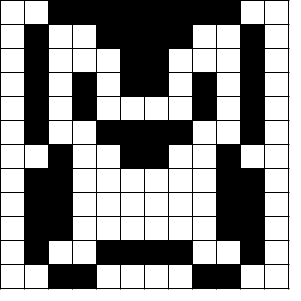
\includegraphics[width=\linewidth]{Pinguin_sw_loesung.png}
\end{minipage}
\begin{minipage}{0.49\linewidth}
	
\includegraphics[width=\linewidth]{Raster_12_12.png}	
\end{minipage}

Beschreibe welche Probleme auftreten, wenn wir Bilder in dieser Form abspeichern.
\liniert[]{4}
\newpage
\aufgabe{}
Die meisten Bilder bestehen aus mehr Farben als nur schwarz und weiß. Übersetze die Zahlenmatrix zurück in ein Bild. Verwende neben weiß und schwarz auch die Farben orange und blau.\\

\begin{minipage}{0.49\linewidth}
	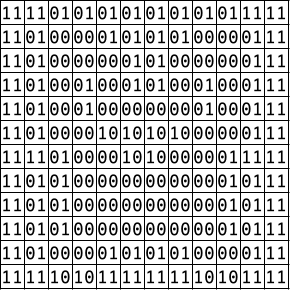
\includegraphics[width=\linewidth]{Pinguin_farbe_matrix.png}
\end{minipage}
\begin{minipage}{0.49\linewidth}
	
\includegraphics[width=\linewidth]{Raster_12_12.png}	
\end{minipage}

\textbf{Tipp: }
\begin{itemize}
	\item \texttt{00} steht für die Farbe weiß.
	\item \texttt{01} steht für die Farbe schwarz.
	\item \texttt{10} steht für die Farbe orange.
	\item \texttt{11} steht für die Farbe blau.
\end{itemize}





%\matheaufgaben{8}{-}

%\input
\label{LastPage}
\normalsize
\ifthenelse{\equal{\TYP}{Klassenarbeit}}{
\input{\patha/Erwartungsbild.tex}}
{}
\ifthenelse{\equal{\TYP}{Leistungskontrolle}}{
\input{\patha/Erwartungsbild.tex}}
{}


\end{document}